\documentclass[11pt, oneside]{article}   	% use "amsart" instead of "article" for AMSLaTeX format
\usepackage{geometry}                		% See geometry.pdf to learn the layout options. There are lots.
\geometry{letterpaper}                   		% ... or a4paper or a5paper or ... 
%\geometry{landscape}                		% Activate for rotated page geometry
%\usepackage[parfill]{parskip}    		% Activate to begin paragraphs with an empty line rather than an indent
\usepackage{graphicx}				% Use pdf, png, jpg, or eps§ with pdflatex; use eps in DVI mode
								% TeX will automatically convert eps --> pdf in pdflatex		
\usepackage{amssymb}

\usepackage{color}
\usepackage{hyperref}
\hypersetup{
    colorlinks,
    citecolor=black,
    filecolor=black,
    linkcolor=black,
    urlcolor=black
}
\usepackage[normalem]{ulem}
\usepackage{fancyhdr}
\fancyhead[L]{December 8, 2015}
\fancyhead[C]{SE 3XA3 Test Plan}
\fancyhead[R]{The A Team}
\pagestyle{fancy}

\usepackage{float}

\usepackage{hyperref}

%SetFonts

%SetFonts


\title{Test Plan}
\author{Gill, Surinder\\
		1308896
		\and
		Hu, Joshua\\
		1311940
		\and
		Lago, Nick\\
		1302613}
\date{December 8, 2015}							% Activate to display a given date or no date

\begin{document}
\maketitle


\newpage
\tableofcontents
\listoffigures
\listoftables

\newpage
\section{Revision History}

\begin{table}[H]
\caption{Revision History: Test Plan}
\begin{center}
\label{tab:}
\begin{tabular}{|c|c|c|c|}
\hline
\textbf{October 21, 2015} & \textbf{DEVELOPER} & \textbf{CHANGE} & \textbf{REVISION}\\
\hline
October 21, 2015 & Gill, Surinder & Sections: 2 & 0\\
\hline
October 21, 2015 & Hu, Joshua & Sections: 3 & 0\\
\hline
October 21, 2015 & Lago, Nick & Sections: 1, 4 & 0\\
\hline
December 7, 2015 & Gill, Surinder & Sections: 1-5 & 1\\
\hline
December 7, 2015 & Hu, Joshua & Sections: 1-5 & 1\\
\hline
December 7, 2015 & Lago, Nick & Sections: 1-5 & 1\\
\hline
\end{tabular}
\end{center}
\label{default}
\end{table}

\newpage
% INTRODUCTION
\section{Introduction}
\subsection{Purpose}
The function of our program is to run a 2D survival arcade style game. This game will have to play sounds, render graphics and interpret user inputs. The testing for this software will include the Jasmine Framework as our automated unit testing. For structural testing our group will implement the Jasmine Framework to test collision detection, user input recognition, and cookie storing.  Functional testing will consist of sound output testing along with sprite rendering and frame resizing. Mutation testing will also occur on our collision detection function as we alter the parameters for optimal sensitivity and to check to make sure that no other function is altered in the process. Fault testing will occur throughout the design and implementation of this project.

\subsection{Environment and Pretest Background}
Since this is a brand new project there has been no previous testing. Since this is similar to a popular game called Flappy Bird we do have expected outputs for all the testing that will occur. 

\subsection{Test Objectives}
Testing will allow our group to make sure that the full functionality of our game is being met. Before releasing our software all of our tests must be thoroughly completed and passed. This grants our team the peace of mind that all functionality of our program is working properly.

\subsection{Expected Defect Rates}
We estimate that no defects will take place during the testing and no further testing will be needed after this set.

\subsection{References}
There is no previously published documentation on this project. There is documentation however on related documents called "Flappy Bird" which should be more than enough: \url{http://flappybird.wikia.com/wiki/Category:Template_documentation}


% PLAN
\section{Plan}
\subsection{Software Description}
%%%%%%%%%%%%%%%%%%%%%%%%%%%%%%
\begin{figure}[H] %  figure placement: here, top, bottom, or page
   \centering
   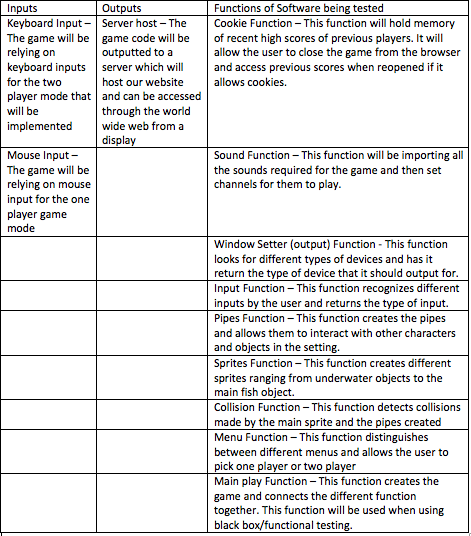
\includegraphics[width=5in]{Table2_SoftwareDescription.png} 
   \caption{Software Description}
   \label{}
\end{figure}%%%%%%%%%%%%%%%%%%%%%%%

\subsection{Test Team}
The test team will consist of Surinder Gill, Nick Lago and Joshua Hu. The three main testers will split the entire testing evenly covering all the different types of testing and preparing the automated testing. 

\subsection{Milestones}
The locations for testing will be centralized in our designated lab locations and work areas. 
Milestones and dates for the testing will be based off the different tests that will be conducted: 
 
 \begin{table}[H]
\caption{Milestones}
\begin{center}
\begin{tabular}{|c|c|}
\hline
\textbf{Module Testing} & \textbf{Expected Date of Completion}\\
\hline
\hline
Sound Output testing & October 30, 2015\\
\hline
Frame resizing testing & October 30, 2015\\
\hline
Input data testing & November 6, 2015\\
\hline
Screen Output (Rendering) testing & November 6, 2015\\
\hline
Sequencing order testing & November 13, 2015\\
\hline
Sprite Rendering testing & November 13, 2015\\
\hline
Cookie storing testing & November 20, 2015\\
\hline
Restart and loop testing & November 20, 2015\\
\hline
\end{tabular}
\end{center}
\label{default}
\end{table}%
 
\subsection{Testing: Primary}
The software that will be required is a JavaScript automated testing framework, a server that can host our website when we're testing on different devices and browsers, a text editor that can make changes to specific pieces of code that will require changing, and a media editor that will be able to modify images and change signs. 
The required personnel to set-up automated testing will be required to have sufficient knowledge in JavaScript and HTML to setup multiple test cases. However, users and development groups that will be doing manual testing do not not have specific requirements needed for testing. 
The automated testing will be done through Jasmine Framework that provides its own documentation. It creates cases that require inputs and expected outputs and will allow the tester to find faults if any. It will create webpages with documentation that show whether a test case has passed or failed and why. 
The proof of concept will indicate correct sound output and frame resizing. It will display a simple test run through the Jasmine Framework showing that both functions are ideal in their outputs. This testing will then be shown and used as a guideline to other tests. 
\\
\\
\\

\subsection{Testing: Secondary}
Secondary testing will be done by users in our open beta testing. We will allow users to access our game at an early development stage after preliminary tests by developers. They will be able to manually perform functional testing by checking for bugs and running through the game through our website. 
\newpage
\section{\textcolor{red}{Structural Testing}}

\subsection{\textcolor{red}{Appearance Testing}}
\textcolor{red}{This will be a structural test by running the game.}
\subsubsection{\textcolor{red}{Test Factors Involved}}
\textcolor{red}{Correctness}
\subsubsection{\textcolor{red}{Initial State}}
\textcolor{red}{Application is running}
\subsubsection{\textcolor{red}{Inputs}}
\textcolor{red}{User inputs}
\subsubsection{\textcolor{red}{Outputs}}
\textcolor{red}{Renders logo, underwater scene background and other entities to catch users eye. }
\subsubsection{\textcolor{red}{Schedule}}
\textcolor{red}{This feature will be implemented for Final Demonstration 1}
\subsubsection{\textcolor{red}{Methodology}}
\textcolor{red}{Tests will be done manually by developers running prototype. Tests will be enhanced by actual user feedback via a survey}
\subsubsection{\textcolor{red}{Test For}}
\textcolor{red}{This test validates section 5.1.1, of requirements documentation.}


\subsection{\textcolor{red}{Style Testing}}
\textcolor{red}{This will be a structural test by running the game.}
\subsubsection{\textcolor{red}{Test Factors Involved}}
\textcolor{red}{Correctness}
\subsubsection{\textcolor{red}{Initial State}}
\textcolor{red}{Application is running}
\subsubsection{\textcolor{red}{Inputs}}
\textcolor{red}{User inputs}
\subsubsection{\textcolor{red}{Outputs}}
\textcolor{red}{Rendering entities to screen}
\subsubsection{\textcolor{red}{Schedule}}
\textcolor{red}{This feature will be implemented for Final Demonstration 1}
\subsubsection{\textcolor{red}{Methodology}}
\textcolor{red}{Tests will be done manually by developers running prototype. Tests will be enhanced by actual user feedback via a survey.}
\subsubsection{\textcolor{red}{Test For}}
\textcolor{red}{This test validates section 5.1.2, of requirements documentation.}



\subsection{\textcolor{red}{Ease of Use Testing}}
\textcolor{red}{This will be a structural test by running the game.}
\subsubsection{\textcolor{red}{Test Factors Involved}}
\textcolor{red}{Ease of Use}
\subsubsection{\textcolor{red}{Initial State}}
\textcolor{red}{Application is running}
\subsubsection{\textcolor{red}{Inputs}}
\textcolor{red}{User inputs}
\subsubsection{\textcolor{red}{Outputs}}
\textcolor{red}{Playability factors based off of users feedback}
\subsubsection{\textcolor{red}{Schedule}}
\textcolor{red}{This feature will be implemented for Final Demonstration 1}
\subsubsection{\textcolor{red}{Methodology}}
\textcolor{red}{Tests will be done manually by developers running prototype. Tests will be enhanced by actual user feedback via a survey.}
\subsubsection{\textcolor{red}{Test For}}
\textcolor{red}{This test validates section 5.1.2, of requirements documentation.}



\subsection{\textcolor{red}{Learning Testing}}
\textcolor{red}{This will be a structural test by running the game.}
\subsubsection{\textcolor{red}{Test Factors Involved}}
\textcolor{red}{Ease of Use}
\subsubsection{\textcolor{red}{Initial State}}
\textcolor{red}{Application is running}
\subsubsection{\textcolor{red}{Inputs}}
\textcolor{red}{User inputs}
\subsubsection{\textcolor{red}{Outputs}}
\textcolor{red}{Ease of use factors made users playing with a mouse}
\subsubsection{\textcolor{red}{Schedule}}
\textcolor{red}{This feature will be implemented for Final Demonstration 1}
\subsubsection{\textcolor{red}{Methodology}}
\textcolor{red}{Tests will be done manually by developers running prototype. Tests will be enhanced by actual user feedback via a survey.}
\subsubsection{\textcolor{red}{Test For}}
\textcolor{red}{This test validates section 5.2.3, of requirements documentation.}



\subsection{\textcolor{red}{Understandability Testing}}
\textcolor{red}{This will be a structural test by running the game.}
\subsubsection{\textcolor{red}{Test Factors Involved}}
\textcolor{red}{Ease of Use}
\subsubsection{\textcolor{red}{Initial State}}
\textcolor{red}{Application is running}
\subsubsection{\textcolor{red}{Inputs}}
\textcolor{red}{User inputs}
\subsubsection{\textcolor{red}{Outputs}}
\textcolor{red}{Understandability factors based off of users feedback}
\subsubsection{\textcolor{red}{Schedule}}
\textcolor{red}{This feature will be implemented for Final Demonstration 1}
\subsubsection{\textcolor{red}{Methodology}}
\textcolor{red}{Tests will be done manually by developers running prototype. Tests will be enhanced by actual user feedback via a survey.}
\subsubsection{\textcolor{red}{Test For}}
\textcolor{red}{This test validates section 5.2.4, of requirements documentation.}



\subsection{\textcolor{red}{Accessibility, and Interfacing with Adjacent Systems Testing}}
\textcolor{red}{This will be a structural test by running the game.}
\subsubsection{\textcolor{red}{Test Factors Involved}}
\textcolor{red}{Ease of Use}
\subsubsection{\textcolor{red}{Initial State}}
\textcolor{red}{Application is activated}
\subsubsection{\textcolor{red}{Inputs}}
\textcolor{red}{Run application on different browsers and devices}
\subsubsection{\textcolor{red}{Outputs}}
\textcolor{red}{Application initialization and playability determined by users}
\subsubsection{\textcolor{red}{Schedule}}
\textcolor{red}{This feature will be implemented for Final Demonstration 1}
\subsubsection{\textcolor{red}{Methodology}}
\textcolor{red}{Tests will be done manually by developers running prototype. Tests will be enhanced by actual user feedback via a survey.}
\subsubsection{\textcolor{red}{Test For}}
\textcolor{red}{This test validates section 5.2.5, and 5.4.2 of requirements documentation.}



\subsection{\textcolor{red}{Speed and Latency Testing}}
\textcolor{red}{This will be a structural test by running the game.}
\subsubsection{\textcolor{red}{Test Factors Involved}}
\textcolor{red}{Ease of Use}
\subsubsection{\textcolor{red}{Initial State}}
\textcolor{red}{Application is activated}
\subsubsection{\textcolor{red}{Inputs}}
\textcolor{red}{User inputs}
\subsubsection{\textcolor{red}{Outputs}}
\textcolor{red}{Application response to user inputs}
\subsubsection{\textcolor{red}{Schedule}}
\textcolor{red}{This feature will be implemented for Final Demonstration 1}
\subsubsection{\textcolor{red}{Methodology}}
\textcolor{red}{Tests will be done manually by developers running prototype. Tests will be enhanced by actual user feedback via a survey.}
\subsubsection{\textcolor{red}{Test For}}
\textcolor{red}{This test validates section 5.3.1, of requirements documentation.}


\subsection{\textcolor{red}{Reliability and Availability, and Expected Physical Environment Testing}}
\textcolor{red}{This will be a structural test by running the game.}
\subsubsection{\textcolor{red}{Test Factors Involved}}
\textcolor{red}{Ease of Use}
\subsubsection{\textcolor{red}{Initial State}}
\textcolor{red}{Application is activated}
\subsubsection{\textcolor{red}{Inputs}}
\textcolor{red}{User to activate game at various locations where access to internet is offered.}
\subsubsection{\textcolor{red}{Outputs}}
\textcolor{red}{Application runs}
\subsubsection{\textcolor{red}{Schedule}}
\textcolor{red}{This feature will be implemented for Final Demonstration 1}
\subsubsection{\textcolor{red}{Methodology}}
\textcolor{red}{Tests will be done manually by developers running prototype. Tests will be enhanced by actual user feedback via a survey.}
\subsubsection{\textcolor{red}{Test For}}
\textcolor{red}{This test validates section 5.3.4 and 5.4.1, of requirements documentation.}



\subsection{\textcolor{red}{Robustness Testing}}
\textcolor{red}{This will be a structural test by running the game.}
\subsubsection{\textcolor{red}{Test Factors Involved}}
\textcolor{red}{Correctness}
\subsubsection{\textcolor{red}{Initial State}}
\textcolor{red}{Application is run}
\subsubsection{\textcolor{red}{Inputs}}
\textcolor{red}{User presses input multiple times in a row.}
\subsubsection{\textcolor{red}{Outputs}}
\textcolor{red}{Application runs smoothly}
\subsubsection{\textcolor{red}{Schedule}}
\textcolor{red}{This feature will be implemented for Final Demonstration 1}
\subsubsection{\textcolor{red}{Methodology}}
\textcolor{red}{Tests will be done manually by developers running prototype. Tests will be enhanced by actual user feedback via a survey.}
\subsubsection{\textcolor{red}{Test For}}
\textcolor{red}{This test validates section 5.3.5, of requirements documentation.}


\subsection{\textcolor{red}{Capacity, and Instability Testing}}
\textcolor{red}{This will be a structural test by running the application.}
\subsubsection{\textcolor{red}{Test Factors Involved}}
\textcolor{red}{Ease of Use}
\subsubsection{\textcolor{red}{Initial State}}
\textcolor{red}{Application is activated}
\subsubsection{\textcolor{red}{Inputs}}
\textcolor{red}{Multiple users will activate application.}
\subsubsection{\textcolor{red}{Outputs}}
\textcolor{red}{Application runs.}
\subsubsection{\textcolor{red}{Schedule}}
\textcolor{red}{This feature will be implemented for Final Demonstration 1}
\subsubsection{\textcolor{red}{Methodology}}
\textcolor{red}{Tests will be done manually by developers running prototype. Tests will be enhanced by actual user feedback via a survey.}
\subsubsection{\textcolor{red}{Test For}}
\textcolor{red}{This test validates section 5.3.6, and 5.3.7of requirements documentation.}


\subsection{\textcolor{red}{Scalability Testing}}
\textcolor{red}{This will be a structural test by running the application.}
\subsubsection{\textcolor{red}{Test Factors Involved}}
\textcolor{red}{Correctness}
\subsubsection{\textcolor{red}{Initial State}}
\textcolor{red}{Application is inactive}
\subsubsection{\textcolor{red}{Inputs}}
\textcolor{red}{Developer will change state variables}
\subsubsection{\textcolor{red}{Outputs}}
\textcolor{red}{Application runs appropriately based on changes to code.}
\subsubsection{\textcolor{red}{Schedule}}
\textcolor{red}{This feature will be implemented for Final Demonstration 1}
\subsubsection{\textcolor{red}{Methodology}}
\textcolor{red}{Tests will be done manually by developers changing code and running the prototype.}
\subsubsection{\textcolor{red}{Test For}}
\textcolor{red}{This test validates section 5.3.8, of requirements documentation.}


\subsection{\textcolor{red}{Longevity Testing}}
\textcolor{red}{This will be a structural test by running the application.}
\subsubsection{\textcolor{red}{Test Factors Involved}}
\textcolor{red}{Correctness}
\subsubsection{\textcolor{red}{Initial State}}
\textcolor{red}{Application is activated}
\subsubsection{\textcolor{red}{Inputs}}
\textcolor{red}{User will play game multiple times in a row without closing browser.}
\subsubsection{\textcolor{red}{Outputs}}
\textcolor{red}{Game runs as expected for entire game time.}
\subsubsection{\textcolor{red}{Schedule}}
\textcolor{red}{This feature will be implemented for Final Demonstration 1}
\subsubsection{\textcolor{red}{Methodology}}
\textcolor{red}{Tests will be done manually by developers running prototype. Tests will be enhanced by actual user feedback via a survey.}
\subsubsection{\textcolor{red}{Test For}}
\textcolor{red}{This test validates section 5.3.9, of requirements documentation.}


\subsection{\textcolor{red}{Productization Testing}}
\textcolor{red}{This will be a structural test by running the application.}
\subsubsection{\textcolor{red}{Test Factors Involved}}
\textcolor{red}{Correctness}
\subsubsection{\textcolor{red}{Initial State}}
\textcolor{red}{Application is activated on developer Surinder's site}
\subsubsection{\textcolor{red}{Inputs}}
\textcolor{red}{Developer will launch game}
\subsubsection{\textcolor{red}{Outputs}}
\textcolor{red}{Application runs as developer deems it should.}
\subsubsection{\textcolor{red}{Schedule}}
\textcolor{red}{This feature will be implemented for Final Demonstration 1}
\subsubsection{\textcolor{red}{Methodology}}
\textcolor{red}{Tests will be done manually by developers running prototype.}
\subsubsection{\textcolor{red}{Test For}}
\textcolor{red}{This test validates section 5.4.3, of requirements documentation.}

\subsection{\textcolor{red}{Supportability, Adaptability and Access Testing}}
\textcolor{red}{This will be a structural test by running the application.}
\subsubsection{\textcolor{red}{Test Factors Involved}}
\textcolor{red}{Correctness}
\subsubsection{\textcolor{red}{Initial State}}
\textcolor{red}{Application is run}
\subsubsection{\textcolor{red}{Inputs}}
\textcolor{red}{Multiple consumers will launch game}
\subsubsection{\textcolor{red}{Outputs}}
\textcolor{red}{Application runs as consumer deems it should.}
\subsubsection{\textcolor{red}{Schedule}}
\textcolor{red}{This feature will be implemented for Final Demonstration 1}
\subsubsection{\textcolor{red}{Methodology}}
\textcolor{red}{Tests will be done manually by consumer running prototype and giving feedback via a survey.}
\subsubsection{\textcolor{red}{Test For}}
\textcolor{red}{This test validates section 5.5.2, 5.5.3 and 5.6.1 of requirements documentation.}


\subsection{\textcolor{red}{Integrity Testing}}
\textcolor{red}{This will be a structural test by running the application.}
\subsubsection{\textcolor{red}{Test Factors Involved}}
\textcolor{red}{Correctness}
\subsubsection{\textcolor{red}{Initial State}}
\textcolor{red}{Application is run}
\subsubsection{\textcolor{red}{Inputs}}
\textcolor{red}{Developer picks garbage inputs}
\subsubsection{\textcolor{red}{Outputs}}
\textcolor{red}{Application does not accept such input.}
\subsubsection{\textcolor{red}{Schedule}}
\textcolor{red}{This feature will be implemented for Final Demonstration 1}
\subsubsection{\textcolor{red}{Methodology}}
\textcolor{red}{Tests will be done manually by consumer running prototype.}
\subsubsection{\textcolor{red}{Test For}}
\textcolor{red}{This test validates section 5.of requirements documentation.}


\subsection{\textcolor{red}{Cultural, Compliance and Standards Testing}}
\textcolor{red}{This will be a structural test by running the application.}
\subsubsection{\textcolor{red}{Test Factors Involved}}
\textcolor{red}{Correctness}
\subsubsection{\textcolor{red}{Initial State}}
\textcolor{red}{Application is run}
\subsubsection{\textcolor{red}{Inputs}}
\textcolor{red}{Developer runs application}
\subsubsection{\textcolor{red}{Outputs}}
\textcolor{red}{No laws, licenses are broken. No cultures are offended.}
\subsubsection{\textcolor{red}{Schedule}}
\textcolor{red}{This feature will be implemented for Final Demonstration 1}
\subsubsection{\textcolor{red}{Methodology}}
\textcolor{red}{Tests will be done manually by consumer running prototype.}
\subsubsection{\textcolor{red}{Test For}}
\textcolor{red}{This test validates section 5.of requirements documentation.}


\newpage
% SPECIFICATIONS AND EVALUATION
\section{Specifications and Evaluation}






\subsubsection*{Business Functions}
\begin{itemize}
\item The executable HTML file will create a new browser window.

\item The HTML will be executed by a browser with JavaScript functionality.

\item The game will have a standby state in which it waits for user input.

\item Upon the reception of user input from the standby state the game will begin.

\item At the beginning of the game the user will perceive all stats reset to their default state.

\item At the beginning of the game the user character will maintain its state until user input is received.

\item If there is a collision with the user character and an obstacle object the game will terminate and all stats will be recorded.

\item Upon termination of the game state all stats will be reset to their default state and the standby state will be reinitiated.

\item If there is a collision with the user character and an objective object the user's score will increment and the objective object's instance will terminate.

\item During the game state reception of user input will cause the user character to respond in a constant and uniform manner relative to the user character's instance.
\end{itemize}

\subsubsection*{Structural Functions}
\begin{itemize}
\item Cookie
\subitem Test how cookies are created and used by the program through static and dynamic testing. This includes code analysis, unit testing, and system testing.

\item Rendering
\subitem Test the use of graphic files compared to drawing objects for the game rendering. This includes manual system testing for aesthetic purposes. 
\end{itemize}

\subsubsection*{Test/Function Relationships}
Much of the testing done for the structural functions will be changed depending on how we (the developers) choose to optimize or design the appearance of the product.\\
\\
For the structural testing of the cookies, it must be decided on which data to store for each cookies instance and how that data will affect the game. This can be done initially through manual code analysis then verified with unit testing, and a manual system test where the value of the cookie can be checked by access through the game and of where the cookies are stored.\\
\\
The structural rendering tests will be used to decide through the aesthetic decisions of the designers and developers the presentation of core functional and ornamental objects in the game. As such the tests conducted will mostly be done through manual system tests although additional unit tests can be performed to validate the functionality of either drawing or using images to render objects.

\subsubsection*{Test Progression}
The tests will proceed by verifying the business functions and all critical components of the project software. With the basis of the project verified structural testing can proceed to optimize the performance of the product and the end users' experience with the product.

\subsection{Methods and Constraints}
\subsubsection*{Methodology}
The A Team's (the developers) approach to testing is to validate the core functionality of the product being developed before testing non-critical components of the product.

\subsubsection*{Test Tools}
For unit testing we will be using the testing framework \href{http://jasmine.github.io/}{Jasmine}. For system testing we will be running the game by executing it on a browser and observing the functionalities. For code analysis we will use humans with coding experience to analyze the code.

\subsubsection*{Extent}
The entirety of the product will be tested.

\subsubsection*{Data Recording}
The results of the unit testing will be written to a test results log. System testing will be added to a separate test log specifcaly for system testing, as will code analysis.\\
\\
All test will contain information on the aspect being tested, the date of the test, the person running the test, the results of the test, a description of the test purpose, a description of the test results, and next steps from the test.

\subsubsection*{Constraints}
Due to the game's simple mechanics, there are few constraints on the testing.

\subsection{Evaluation}
\subsubsection*{Criteria}
Our tests will cover primarily the boundaries of the game mechanics and some testing inside the boundaries as an example test of normal behaviour.

\subsubsection*{Data Reduction}
All test logs will indicate a pass or a need fro review which allow us to focus on reimplementing and testing components which do not pass the tests.

\newpage
% TEST DESCRIPTION
\section{Test Descriptions}
\subsection{Test Identification}
Control: The team are going to be using automatic insertions, in the form of a unit tester named Jasmine. Our team will also manually create non automated inputs in the form of playing the game.\\
\\
\sout{The inputs created from Jasmine will be in the three different forms. First will we have Jasmine change the location of our fish player to random locations, and by knowing what spaces are occupied by pipes, the Jasmine Framework can determine when the collision function should return true. Next our inputs will be in the form of Jasmine checking for stored cookies. As a result of some browsers not allowing cookies, this isn't a full proof test and some manual testing will be needed. Lastly, the input going into the input recognition function will be a replica of random inputs a user may put if they were actually playing. If the program registers the input as intended, the program will pass. For the manual testing, our inputs will be the team actually running the game and giving usual and unusual user inputs and seeing how the program reacts.}\\
 \\
Manual testing will occur on different browsers such as Chrome, Explorer, Firefox, etc. This will allow diversity within our tests. Automated testing (through Jasmine) will consist of many different sets of inputs. Jasmine will be given a set of expected outputs and will allow a test to pass if these outputs are met given many different inputs. Some tests will attempt to generate exceptions by accessing inputs outside of the alphabet of possible inputs such as accessing cookies that do not exist, etc.\\
\\
\sout{The outputs will be pretty straight forward to tell for the Jasmine Framework. If the fish is on the same location that is occupied by a pipe the collision function should return true. The output for the cookie testing will be slightly different, as it will just be a check to see if the cookies were stored. The output for our manual testing will be comprised of images showing the expected results}.

\subsection{Additional Test Identification}
The last of our testing will be semantics and syntax testing. We need for this program to render neatly and look clean. This will be done by trying different frame sizes, different animations and changing the images in our sprite library. Checking this fairly regularly is a smart idea to find the most ascetically pleasing set of sprites and the nicest size to fit our game onto (a preferred size). Variable naming and implementation layouts will be tested to make sure our code is understandable to all members and that the code makes sense to someone trying to maintain it. Syntax will be tested regularly by running the program and having other members look over new additions. This will make sure that we avoid a syntax mistake that could cause problems later down the road for our project and have the team unsure about its location. System tests will be conducted to cross check against the prototype to ensure proper functionality.\\
\\
In addition structural testing will include performance, difficulty, accessibility, and meeting aesthetic requirements. Performance related testing will determine frame rate speeds on differing browsers; server lag and the machine's processing power will be taken into consideration. Difficulty will be adjusted for a subjectively optimal user experience by mutation testing the rendered obstacle functions. The accessibility will be tested by running system tests on different machine types running varying browsers and operating systems per test. Aesthetic requirements will be met through manual system testing by using different sprite designs and will be decided at the discretion of the developers.


\section{\textcolor{red}{Unit-Testing}}

\subsection{\textcolor{red}{Cookie Handler Setter Testing}}
\textcolor{red}{This will be a unit test using Jasmine Framework to validate correctness.}
\subsubsection{\textcolor{red}{Test Factors Involved}}
\textcolor{red}{Correctness}
\subsubsection{\textcolor{red}{Initial State}}
\textcolor{red}{No cookies stored at the moment}
\subsubsection{\textcolor{red}{Inputs}}
\textcolor{red}{Entering in the website address hosting the application. A  cookie will be inserted that has a name, value and expiry date.}
\subsubsection{\textcolor{red}{Outputs}}
\textcolor{red}{A cookie will be stored on the user's browser that contains.}

\subsubsection{\textcolor{red}{Schedule}}
\textcolor{red}{This test regards the main simulation of the game and therefore will be necessary for the Final Demonstration 1}
\subsubsection{\textcolor{red}{Methodology}}
\textcolor{red}{This test will be conducted by setting a new cookie using the setCookie method in the cookies class. It will be conducted through the Jasmine Framework and outputted in our unit test HTML file}
\subsubsection{\textcolor{red}{Tests For}}
\textcolor{red}{This test validates section 4.4.1, of requirements documentation.}



\subsection{\textcolor{red}{Cookie Handler Checker Testing}}
\textcolor{red}{This will be a unit test using Jasmine Framework to validate correctness.}
\subsubsection{\textcolor{red}{Test Factors Involved}}
\textcolor{red}{Correctness}
\subsubsection{\textcolor{red}{Initial State}}
\textcolor{red}{No cookies stored at the moment}
\subsubsection{\textcolor{red}{Inputs}}
\textcolor{red}{Entering in the website address hosting the application. A cookie will be inserted that has a name, value of 2 and expiry date.}
\subsubsection{\textcolor{red}{Outputs}}
\textcolor{red}{A cookie will be checked to see if there is a value of 2.}
\subsubsection{\textcolor{red}{Schedule}}
\textcolor{red}{This test regards the main simulation of the game and therefore will be necessary for the Final Demonstration 1}
\subsubsection{\textcolor{red}{Methodology}}
\textcolor{red}{This test will be conducted by setting a new cookie using the setCookie method and equals in the cookies class. It will be conducted through the Jasmine Framework and outputted in our unit test HTML file}
\subsubsection{\textcolor{red}{Tests For}}
\textcolor{red}{This test validates section 4.4.1, of requirements documentation.}



\subsection{\textcolor{red}{Cookie Handler Getter Testing}}
\textcolor{red}{This will be a unit test using Jasmine Framework to validate correctness.}
\subsubsection{\textcolor{red}{Test Factors Involved}}
\textcolor{red}{Correctness}
\subsubsection{\textcolor{red}{Initial State}}
\textcolor{red}{Cookie stored with a value of 42.}
\subsubsection{\textcolor{red}{Inputs}}
\textcolor{red}{Entering in the website address hosting the application. }
\subsubsection{\textcolor{red}{Outputs}}
\textcolor{red}{A cookie will be checked that has a name, value of 42 and expiry date.}
\subsubsection{\textcolor{red}{Schedule}}
\textcolor{red}{This test regards the main simulation of the game and therefore will be necessary for the Final Demonstration 1}
\subsubsection{\textcolor{red}{Methodology}}
\textcolor{red}{This test will be conducted by setting a new cookie using the getCookie method and equals in the cookies class. It will be conducted through the Jasmine Framework and outputted in our unit test HTML file}
\subsubsection{\textcolor{red}{Tests For}}
\textcolor{red}{This test validates section 4.4.2, of requirements documentation.}


\subsection{\textcolor{red}{Cookie Handler Getter Testing}}
\textcolor{red}{This will be a unit test using Jasmine Framework to validate correctness.}
\subsubsection{\textcolor{red}{Test Factors Involved}}
\textcolor{red}{Correctness}
\subsubsection{\textcolor{red}{Initial State}}
\textcolor{red}{Cookie stored with a value of 42.}
\subsubsection{\textcolor{red}{Inputs}}
\textcolor{red}{Entering in the website address hosting the application. }
\subsubsection{\textcolor{red}{Outputs}}
\textcolor{red}{A cookie will be checked that has a name, null value and expiry date.}
\subsubsection{\textcolor{red}{Schedule}}
\textcolor{red}{This test regards the main simulation of the game and therefore will be necessary for the Final Demonstration 1}
\subsubsection{\textcolor{red}{Methodology}}
\textcolor{red}{This test will be conducted by setting a new cookie using the getCookie method and equals in the cookies class. It will be conducted through the Jasmine Framework and outputted in our unit test HTML file}
\subsubsection{\textcolor{red}{Tests For}}
\textcolor{red}{This test validates section 4.4.2, of requirements documentation.}



\subsection{\textcolor{red}{Background Content Testing}}
\textcolor{red}{This will be a unit test using Jasmine Framework to validate correctness.}
\subsubsection{\textcolor{red}{Test Factors Involved}}
\textcolor{red}{Correctness}
\subsubsection{\textcolor{red}{Initial State}}
\textcolor{red}{this.bg is initialized}
\subsubsection{\textcolor{red}{Inputs}}
\textcolor{red}{Input this.bg.src = bg.png from files}
\subsubsection{\textcolor{red}{Outputs}}
\textcolor{red}{Check to see if bg has an image attached to it.}
\subsubsection{\textcolor{red}{Schedule}}
\textcolor{red}{This test regards the main simulation of the game and therefore will be necessary for the Final Demonstration 1}
\subsubsection{\textcolor{red}{Methodology}}
\textcolor{red}{This test will be conducted by setting a picture to the background and check to see if it has done that. It will be conducted through the Jasmine Framework and outputted in our unit test HTML file}
\subsubsection{\textcolor{red}{Tests For}}
\textcolor{red}{This test validates section 4.4.13, of requirements documentation.}



\subsection{\textcolor{red}{Background Coordinate Testing}}
\textcolor{red}{This will be a unit test using Jasmine Framework to validate correctness.}
\subsubsection{\textcolor{red}{Test Factors Involved}}
\textcolor{red}{Correctness}
\subsubsection{\textcolor{red}{Initial State}}
\textcolor{red}{this.x and this.y is initialized}
\subsubsection{\textcolor{red}{Inputs}}
\textcolor{red}{Inputs: x-coordinate, y-coordinate and radius}
\subsubsection{\textcolor{red}{Outputs}}
\textcolor{red}{Check to see if inputs have the correct x and y coordinates.}
\subsubsection{\textcolor{red}{Schedule}}
\textcolor{red}{This test regards the main simulation of the game and therefore will be necessary for the Final Demonstration 1}
\subsubsection{\textcolor{red}{Methodology}}
\textcolor{red}{This test will be conducted by checking for the inputs from the bottomBar function and checking to see if they are correct. It will be conducted through the Jasmine Framework and outputted in our unit test HTML file}
\subsubsection{\textcolor{red}{Tests For}}
\textcolor{red}{This test validates section 4.4.13, of requirements documentation.}





\subsection{\textcolor{red}{Collision Particle Testing}}
\textcolor{red}{This will be a unit test using Jasmine Framework to validate correctness.}
\subsubsection{\textcolor{red}{Test Factors Involved}}
\textcolor{red}{Correctness}
\subsubsection{\textcolor{red}{Initial State}}
\textcolor{red}{Coordinates for fish have been initialized}
\subsubsection{\textcolor{red}{Inputs}}
\textcolor{red}{Inputs: fish and pipe objects}
\subsubsection{\textcolor{red}{Outputs}}
\textcolor{red}{Check to see if x and y coordinates of the fish are in contact with the x and y coordinates of the pipe.}
\subsubsection{\textcolor{red}{Schedule}}
\textcolor{red}{This test regards the main simulation of the game and therefore will be necessary for the Final Demonstration 1}
\subsubsection{\textcolor{red}{Methodology}}
\textcolor{red}{This test will be conducted by checking for the inputs from the collides function and checking to see if they interact. It will be conducted through the Jasmine Framework and outputted in our unit test HTML file}
\subsubsection{\textcolor{red}{Tests For}}
\textcolor{red}{This test validates section 4.4.9, of requirements documentation.}




\subsection{\textcolor{red}{Collision Matching Testing}}
\textcolor{red}{This will be a unit test using Jasmine Framework to validate correctness.}
\subsubsection{\textcolor{red}{Test Factors Involved}}
\textcolor{red}{Correctness}
\subsubsection{\textcolor{red}{Initial State}}
\textcolor{red}{Coordinates for fish and pipe have been initialized}
\subsubsection{\textcolor{red}{Inputs}}
\textcolor{red}{Inputs: fish and pipe objects}
\subsubsection{\textcolor{red}{Outputs}}
\textcolor{red}{Check to see if x and y coordinates of the fish are in distance with the x and y coordinates of the pipe.}
\subsubsection{\textcolor{red}{Schedule}}
\textcolor{red}{This test regards the main simulation of the game and therefore will be necessary for the Final Demonstration 1}
\subsubsection{\textcolor{red}{Methodology}}
\textcolor{red}{This test will be conducted by checking for the inputs from the collides function and checking to see if they are in contact. It will be conducted through the Jasmine Framework and outputted in our unit test HTML file}
\subsubsection{\textcolor{red}{Tests For}}
\textcolor{red}{This test validates section 4.4.9, of requirements documentation.}



\subsection{\textcolor{red}{Collision Null Testing}}
\textcolor{red}{This will be a unit test using Jasmine Framework to validate correctness.}
\subsubsection{\textcolor{red}{Test Factors Involved}}
\textcolor{red}{Correctness}
\subsubsection{\textcolor{red}{Initial State}}
\textcolor{red}{Coordinates for fish and pipe have been initialized}
\subsubsection{\textcolor{red}{Inputs}}
\textcolor{red}{Inputs: fish and pipe objects}
\subsubsection{\textcolor{red}{Outputs}}
\textcolor{red}{Check to see if the collision is null because there is no collision occurring.}
\subsubsection{\textcolor{red}{Schedule}}
\textcolor{red}{This test regards the main simulation of the game and therefore will be necessary for the Final Demonstration 1}
\subsubsection{\textcolor{red}{Methodology}}
\textcolor{red}{This test will be conducted by checking for the inputs from the collides function and confirming that a null is correct. It will be conducted through the Jasmine Framework and outputted in our unit test HTML file}
\subsubsection{\textcolor{red}{Tests For}}
\textcolor{red}{This test validates section 4.4.9, of requirements documentation.}




\subsection{\textcolor{red}{PowerUp Collision Particle Testing}}
\textcolor{red}{This will be a unit test using Jasmine Framework to validate correctness.}
\subsubsection{\textcolor{red}{Test Factors Involved}}
\textcolor{red}{Correctness}
\subsubsection{\textcolor{red}{Initial State}}
\textcolor{red}{Coordinates for fish and powerup have been initialized}
\subsubsection{\textcolor{red}{Inputs}}
\textcolor{red}{Inputs: fish and powerup objects}
\subsubsection{\textcolor{red}{Outputs}}
\textcolor{red}{Check to see if x and y coordinates of the fish are in contact with the x and y coordinates of the powerup.}
\subsubsection{\textcolor{red}{Schedule}}
\textcolor{red}{This test regards the main simulation of the game and therefore will be necessary for the Final Demonstration 1}
\subsubsection{\textcolor{red}{Methodology}}
\textcolor{red}{This test will be conducted by checking for the inputs from the powerup collides function and checking to see if they interact. It will be conducted through the Jasmine Framework and outputted in our unit test HTML file}
\subsubsection{\textcolor{red}{Tests For}}
\textcolor{red}{This test validates section 4.4.9, of requirements documentation.}




\subsection{\textcolor{red}{PowerUp Collision Matching Testing}}
\textcolor{red}{This will be a unit test using Jasmine Framework to validate correctness.}
\subsubsection{\textcolor{red}{Test Factors Involved}}
\textcolor{red}{Correctness}
\subsubsection{\textcolor{red}{Initial State}}
\textcolor{red}{Coordinates for fish and powerup have been initialized}
\subsubsection{\textcolor{red}{Inputs}}
\textcolor{red}{Inputs: fish and powerup objects}
\subsubsection{\textcolor{red}{Outputs}}
\textcolor{red}{Check to see if x and y coordinates of the fish are in distance with the x and y coordinates of the powerup.}
\subsubsection{\textcolor{red}{Schedule}}
\textcolor{red}{This test regards the main simulation of the game and therefore will be necessary for the Final Demonstration 1}
\subsubsection{\textcolor{red}{Methodology}}
\textcolor{red}{This test will be conducted by checking for the inputs from the powerup collides function and checking to see if they are in contact. It will be conducted through the Jasmine Framework and outputted in our unit test HTML file}
\subsubsection{\textcolor{red}{Tests For}}
\textcolor{red}{This test validates section 4.4.9, of requirements documentation.}



\subsection{\textcolor{red}{PowerUp Collision Null Testing}}
\textcolor{red}{This will be a unit test using Jasmine Framework to validate correctness.}
\subsubsection{\textcolor{red}{Test Factors Involved}}
\textcolor{red}{Correctness}
\subsubsection{\textcolor{red}{Initial State}}
\textcolor{red}{Coordinates for fish and pipe have been initialized}
\subsubsection{\textcolor{red}{Inputs}}
\textcolor{red}{Inputs: fish and pipe objects}
\subsubsection{\textcolor{red}{Outputs}}
\textcolor{red}{Check to see if the collision is null because there is no collision occurring.}
\subsubsection{\textcolor{red}{Schedule}}
\textcolor{red}{This test regards the main simulation of the game and therefore will be necessary for the Final Demonstration 1}
\subsubsection{\textcolor{red}{Methodology}}
\textcolor{red}{This test will be conducted by checking for the inputs from the collides function and confirming that a null is correct. It will be conducted through the Jasmine Framework and outputted in our unit test HTML file}
\subsubsection{\textcolor{red}{Tests For}}
\textcolor{red}{This test validates section 4.4.9, of requirements documentation.}


\subsection{\textcolor{red}{Draw Rectangle Testing}}
\textcolor{red}{This will be a unit test using Jasmine Framework to validate correctness.}
\subsubsection{\textcolor{red}{Test Factors Involved}}
\textcolor{red}{Correctness}
\subsubsection{\textcolor{red}{Initial State}}
\textcolor{red}{N/A}
\subsubsection{\textcolor{red}{Inputs}}
\textcolor{red}{Inputs: x, y, width, height, colour}
\subsubsection{\textcolor{red}{Outputs}}
\textcolor{red}{Check to see if the object is filled with the colour and appropriate dimensions.}
\subsubsection{\textcolor{red}{Schedule}}
\textcolor{red}{This test regards the main simulation of the game and therefore will be necessary for the Final Demonstration 1}
\subsubsection{\textcolor{red}{Methodology}}
\textcolor{red}{This test will be conducted by comparing the inputs from the draw rect function and confirming that all the variables have recieved the inputs. It will be conducted through the Jasmine Framework and outputted in our unit test HTML file}
\subsubsection{\textcolor{red}{Tests For}}
\textcolor{red}{This test validates section 4.4.14, of requirements documentation.}



\subsection{\textcolor{red}{Draw Circle Testing}}
\textcolor{red}{This will be a unit test using Jasmine Framework to validate correctness.}
\subsubsection{\textcolor{red}{Test Factors Involved}}
\textcolor{red}{Correctness}
\subsubsection{\textcolor{red}{Initial State}}
\textcolor{red}{N/A}
\subsubsection{\textcolor{red}{Inputs}}
\textcolor{red}{Inputs: x, y, radius, colour}
\subsubsection{\textcolor{red}{Outputs}}
\textcolor{red}{Check to see if the object is filled with the colour and appropriate dimensions.}
\subsubsection{\textcolor{red}{Schedule}}
\textcolor{red}{This test regards the main simulation of the game and therefore will be necessary for the Final Demonstration 1}
\subsubsection{\textcolor{red}{Methodology}}
\textcolor{red}{This test will be conducted by comparing the inputs from the draw circle function and confirming that all the variables have received the inputs. It will be conducted through the Jasmine Framework and outputted in our unit test HTML file}
\subsubsection{\textcolor{red}{Tests For}}
\textcolor{red}{This test validates section 4.4.14, of requirements documentation.}



\subsection{\textcolor{red}{Draw Image Testing}}
\textcolor{red}{This will be a unit test using Jasmine Framework to validate correctness.}
\subsubsection{\textcolor{red}{Test Factors Involved}}
\textcolor{red}{Correctness}
\subsubsection{\textcolor{red}{Initial State}}
\textcolor{red}{N/A}
\subsubsection{\textcolor{red}{Inputs}}
\textcolor{red}{Inputs: x, y, img}
\subsubsection{\textcolor{red}{Outputs}}
\textcolor{red}{Check to see if the object has loaded the correct image and appropriate dimensions.}
\subsubsection{\textcolor{red}{Schedule}}
\textcolor{red}{This test regards the main simulation of the game and therefore will be necessary for the Final Demonstration 1}
\subsubsection{\textcolor{red}{Methodology}}
\textcolor{red}{This test will be conducted by comparing the inputs from the draw image function and confirming that all the variables have recieved the inputs. It will be conducted through the Jasmine Framework and outputted in our unit test HTML file}
\subsubsection{\textcolor{red}{Tests For}}
\textcolor{red}{This test validates section 4.4.14, of requirements documentation.}



\subsection{\textcolor{red}{Draw Sprite Testing}}
\textcolor{red}{This will be a unit test using Jasmine Framework to validate correctness.}
\subsubsection{\textcolor{red}{Test Factors Involved}}
\textcolor{red}{Correctness}
\subsubsection{\textcolor{red}{Initial State}}
\textcolor{red}{N/A}
\subsubsection{\textcolor{red}{Inputs}}
\textcolor{red}{Inputs: img, srcX, srcY, srcW, srcH, destX, destY, destW, destH, r}
\subsubsection{\textcolor{red}{Outputs}}
\textcolor{red}{Check to see if the object has loaded the correct image and appropriate dimensions.}
\subsubsection{\textcolor{red}{Schedule}}
\textcolor{red}{This test regards the main simulation of the game and therefore will be necessary for the Final Demonstration 1}
\subsubsection{\textcolor{red}{Methodology}}
\textcolor{red}{This test will be conducted by comparing the inputs from the draw sprite function and confirming that all the variables have recieved the inputs. It will be conducted through the Jasmine Framework and outputted in our unit test HTML file}
\subsubsection{\textcolor{red}{Tests For}}
\textcolor{red}{This test validates section 4.4.14, of requirements documentation.}


\subsection{\textcolor{red}{Draw Text Testing}}
\textcolor{red}{This will be a unit test using Jasmine Framework to validate correctness.}
\subsubsection{\textcolor{red}{Test Factors Involved}}
\textcolor{red}{Correctness}
\subsubsection{\textcolor{red}{Initial State}}
\textcolor{red}{N/A}
\subsubsection{\textcolor{red}{Inputs}}
\textcolor{red}{Inputs: string, x, y, size, colour}
\subsubsection{\textcolor{red}{Outputs}}
\textcolor{red}{Check to see if the object has loaded the correct image, colour and appropriate dimensions.}
\subsubsection{\textcolor{red}{Schedule}}
\textcolor{red}{This test regards the main simulation of the game and therefore will be necessary for the Final Demonstration 1}
\subsubsection{\textcolor{red}{Methodology}}
\textcolor{red}{This test will be conducted by comparing the inputs from the draw text function and confirming that all the variables have recieved the inputs. It will be conducted through the Jasmine Framework and outputted in our unit test HTML file}
\subsubsection{\textcolor{red}{Tests For}}
\textcolor{red}{This test validates section 4.4.14, of requirements documentation.}


\subsection{\textcolor{red}{Fish Image Function Testing}}
\textcolor{red}{This will be a unit test using Jasmine Framework to validate correctness.}
\subsubsection{\textcolor{red}{Test Factors Involved}}
\textcolor{red}{Correctness}
\subsubsection{\textcolor{red}{Initial State}}
\textcolor{red}{N/A}
\subsubsection{\textcolor{red}{Inputs}}
\textcolor{red}{There are no inputs}
\subsubsection{\textcolor{red}{Outputs}}
\textcolor{red}{Check to see if the image is initialized and loaded.}
\subsubsection{\textcolor{red}{Schedule}}
\textcolor{red}{This test regards the main simulation of the game and therefore will be necessary for the Final Demonstration 1}
\subsubsection{\textcolor{red}{Methodology}}
 It will be conducted through the Jasmine Framework and outputted in our unit test HTML file}
\subsubsection{\textcolor{red}{Tests For}}
\textcolor{red}{This test validates section 4.4.13, of requirements documentation.}



\subsection{\textcolor{red}{Fish Gravity Function Testing}}
\textcolor{red}{This will be a unit test using Jasmine Framework to validate correctness.}
\subsubsection{\textcolor{red}{Test Factors Involved}}
\textcolor{red}{Correctness}
\subsubsection{\textcolor{red}{Initial State}}
\textcolor{red}{N/A}
\subsubsection{\textcolor{red}{Inputs}}
\textcolor{red}{There are no inputs}
\subsubsection{\textcolor{red}{Outputs}}
\textcolor{red}{Check to see if gravity is initialized and set to default value.}
\subsubsection{\textcolor{red}{Schedule}}
\textcolor{red}{This test regards the main simulation of the game and therefore will be necessary for the Final Demonstration 1}
\subsubsection{\textcolor{red}{Methodology}}
\textcolor{red}{This test will be conducted by initializing gravity and giving it a default value set by the developer. It will be conducted through the Jasmine Framework and outputted in our unit test HTML file}
\subsubsection{\textcolor{red}{Tests For}}
\textcolor{red}{This test validates section 4.4.16, of requirements documentation.}



\subsection{\textcolor{red}{Fish Velocity Function Testing}}
\textcolor{red}{This will be a unit test using Jasmine Framework to validate correctness.}
\subsubsection{\textcolor{red}{Test Factors Involved}}
\textcolor{red}{Correctness}
\subsubsection{\textcolor{red}{Initial State}}
\textcolor{red}{N/A}
\subsubsection{\textcolor{red}{Inputs}}
\textcolor{red}{There are no inputs}
\subsubsection{\textcolor{red}{Outputs}}
\textcolor{red}{Check to see if velocity is initialized and set to default value.}
\subsubsection{\textcolor{red}{Schedule}}
\textcolor{red}{This test regards the main simulation of the game and therefore will be necessary for the Final Demonstration 1}
\subsubsection{\textcolor{red}{Methodology}}
\textcolor{red}{This test will be conducted by initializing velocity and giving it a default value set by the developer. It will be conducted through the Jasmine Framework and outputted in our unit test HTML file}
\subsubsection{\textcolor{red}{Tests For}}
\textcolor{red}{This test validates section 4.4.16, of requirements documentation.}


\subsection{\textcolor{red}{User Input Tap Testing}}
\textcolor{red}{This will be a unit test using Jasmine Framework to validate correctness.}
\subsubsection{\textcolor{red}{Test Factors Involved}}
\textcolor{red}{Correctness}
\subsubsection{\textcolor{red}{Initial State}}
\textcolor{red}{N/A}
\subsubsection{\textcolor{red}{Inputs}}
\textcolor{red}{Input: User click or tap}
\subsubsection{\textcolor{red}{Outputs}}
\textcolor{red}{Check to see if user has clicked on the window.}
\subsubsection{\textcolor{red}{Schedule}}
\textcolor{red}{This test regards the main simulation of the game and therefore will be necessary for the Final Demonstration 1}
\subsubsection{\textcolor{red}{Methodology}}
\textcolor{red}{This test will be conducted by checking to see if the user click is not null. It will be conducted through the Jasmine Framework and outputted in our unit test HTML file}
\subsubsection{\textcolor{red}{Tests For}}
\textcolor{red}{This test validates section 4.4.12, of requirements documentation.}



\subsection{\textcolor{red}{Jump Buffer Testing}}
\textcolor{red}{This will be a unit test using Jasmine Framework to validate correctness.}
\subsubsection{\textcolor{red}{Test Factors Involved}}
\textcolor{red}{Correctness}
\subsubsection{\textcolor{red}{Initial State}}
\textcolor{red}{N/A}
\subsubsection{\textcolor{red}{Inputs}}
\textcolor{red}{There are no inputs.}
\subsubsection{\textcolor{red}{Outputs}}
\textcolor{red}{Check that the jump buffer is set to -3.}
\subsubsection{\textcolor{red}{Schedule}}
\textcolor{red}{This test regards the main simulation of the game and therefore will be necessary for the Final Demonstration 1}
\subsubsection{\textcolor{red}{Methodology}}
\textcolor{red}{This test will be conducted by checking to see if the jump buffer is set to -3 but the equals function in Jasmine. It will be conducted through the Jasmine Framework and outputted in our unit test HTML file}
\subsubsection{\textcolor{red}{Tests For}}
\textcolor{red}{This test validates section 4.4.16, of requirements documentation.}



\subsection{\textcolor{red}{Medal Object Testing}}
\textcolor{red}{This will be a unit test using Jasmine Framework to validate correctness.}
\subsubsection{\textcolor{red}{Test Factors Involved}}
\textcolor{red}{Correctness}
\subsubsection{\textcolor{red}{Initial State}}
\textcolor{red}{N/A}
\subsubsection{\textcolor{red}{Inputs}}
\textcolor{red}{The user's score.}
\subsubsection{\textcolor{red}{Outputs}}
\textcolor{red}{The medal colour based on score.}
\subsubsection{\textcolor{red}{Schedule}}
\textcolor{red}{This test regards the main simulation of the game and therefore will be necessary for the Final Demonstration 1}
\subsubsection{\textcolor{red}{Methodology}}
\textcolor{red}{This test will be conducted by checking to see if the correct medal is returned from GameOver function. It will be conducted through the Jasmine Framework and outputted in our unit test HTML file}
\subsubsection{\textcolor{red}{Tests For}}
\textcolor{red}{This test validates section 4.4.13, of requirements documentation.}


\subsection{\textcolor{red}{Correct Play Again Inputs Testing}}
\textcolor{red}{This will be a unit test using Jasmine Framework to validate correctness.}
\subsubsection{\textcolor{red}{Test Factors Involved}}
\textcolor{red}{Correctness}
\subsubsection{\textcolor{red}{Initial State}}
\textcolor{red}{GameOver Mode}
\subsubsection{\textcolor{red}{Inputs}}
\textcolor{red}{Input: x and y coordinates}
\subsubsection{\textcolor{red}{Outputs}}
\textcolor{red}{Update to restart game.}
\subsubsection{\textcolor{red}{Schedule}}
\textcolor{red}{This test regards the main simulation of the game and therefore will be necessary for the Final Demonstration 1}
\subsubsection{\textcolor{red}{Methodology}}
\textcolor{red}{This test will be conducted by checking to see if the user has tapped within a certain area to restart the game. It will be conducted through the Jasmine Framework and outputted in our unit test HTML file}
\subsubsection{\textcolor{red}{Tests For}}
\textcolor{red}{This test validates section 4.4.10 and 4.4.11, of requirements documentation.}


\subsection{\textcolor{red}{Cookie Access Testing}}
\textcolor{red}{This will be a unit test using Jasmine Framework to validate correctness.}
\subsubsection{\textcolor{red}{Test Factors Involved}}
\textcolor{red}{Correctness}
\subsubsection{\textcolor{red}{Initial State}}
\textcolor{red}{GameOver Mode}
\subsubsection{\textcolor{red}{Inputs}}
\textcolor{red}{Input: User's Highscore}
\subsubsection{\textcolor{red}{Outputs}}
\textcolor{red}{New Highscore when old highscore is lower}
\subsubsection{\textcolor{red}{Schedule}}
\textcolor{red}{This test regards the main simulation of the game and therefore will be necessary for the Final Demonstration 1}
\subsubsection{\textcolor{red}{Methodology}}
\textcolor{red}{This test will be conducted by making the highscore bigger and checking to see if it has changed. It will be conducted through the Jasmine Framework and outputted in our unit test HTML file}
\subsubsection{\textcolor{red}{Tests For}}
\textcolor{red}{This test validates section 4.4.2, of requirements documentation.}


\subsection{\textcolor{red}{Input Testing}}
\textcolor{red}{This will be a unit test using Jasmine Framework to validate correctness.}
\subsubsection{\textcolor{red}{Test Factors Involved}}
\textcolor{red}{Correctness}
\subsubsection{\textcolor{red}{Initial State}}
\textcolor{red}{Game Running State}
\subsubsection{\textcolor{red}{Inputs}}
\textcolor{red}{Input: User's mouse click}
\subsubsection{\textcolor{red}{Outputs}}
\textcolor{red}{X and y coordinates from the user's mouse click.}
\subsubsection{\textcolor{red}{Schedule}}
\textcolor{red}{This test regards the main simulation of the game and therefore will be necessary for the Final Demonstration 1}
\subsubsection{\textcolor{red}{Methodology}}
\textcolor{red}{This test will be conducted by confirming that the user's click is recorded in x and y values. It will be conducted through the Jasmine Framework and outputted in our unit test HTML file}
\subsubsection{\textcolor{red}{Tests For}}
\textcolor{red}{This test validates section 4.4.12, of requirements documentation.}



\subsection{\textcolor{red}{Input Null Testing}}
\textcolor{red}{This will be a unit test using Jasmine Framework to validate correctness.}
\subsubsection{\textcolor{red}{Test Factors Involved}}
\textcolor{red}{Correctness}
\subsubsection{\textcolor{red}{Initial State}}
\textcolor{red}{Game Running State}
\subsubsection{\textcolor{red}{Inputs}}
\textcolor{red}{Input: User's mouse click}
\subsubsection{\textcolor{red}{Outputs}}
\textcolor{red}{Null checker for user's mouse click.}
\subsubsection{\textcolor{red}{Schedule}}
\textcolor{red}{This test regards the main simulation of the game and therefore will be necessary for the Final Demonstration 1}
\subsubsection{\textcolor{red}{Methodology}}
\textcolor{red}{This test will be conducted by confirming that the user's click is not null during the click. It will be conducted through the Jasmine Framework and outputted in our unit test HTML file}
\subsubsection{\textcolor{red}{Tests For}}
\textcolor{red}{This test validates section 4.4.12, of requirements documentation.}


\subsection{\textcolor{red}{Coin Testing}}
\textcolor{red}{This will be a unit test using Jasmine Framework to validate correctness.}
\subsubsection{\textcolor{red}{Test Factors Involved}}
\textcolor{red}{Correctness}
\subsubsection{\textcolor{red}{Initial State}}
\textcolor{red}{Game Running State}
\subsubsection{\textcolor{red}{Inputs}}
\textcolor{red}{There is no input}
\subsubsection{\textcolor{red}{Outputs}}
\textcolor{red}{Location of coin in retrospect to pipe}
\subsubsection{\textcolor{red}{Schedule}}
\textcolor{red}{This test regards the main simulation of the game and therefore will be necessary for the Final Demonstration 1}
\subsubsection{\textcolor{red}{Methodology}}
\textcolor{red}{This test will be conducted by assessing the location of the coin in the frame based off coordinates. It will be conducted through the Jasmine Framework and outputted in our unit test HTML file}
\subsubsection{\textcolor{red}{Tests For}}
\textcolor{red}{This test validates section 4.4.13, of requirements documentation.}


\subsection{\textcolor{red}{Image Rendering Testing}}
\textcolor{red}{This will be a unit test using Jasmine Framework to validate correctness.}
\subsubsection{\textcolor{red}{Test Factors Involved}}
\textcolor{red}{Correctness}
\subsubsection{\textcolor{red}{Initial State}}
\textcolor{red}{Game Running State}
\subsubsection{\textcolor{red}{Inputs}}
\textcolor{red}{Input: Source image from root folders.}
\subsubsection{\textcolor{red}{Outputs}}
\textcolor{red}{Variables are assigned to particular images and have been initialized.}
\subsubsection{\textcolor{red}{Schedule}}
\textcolor{red}{This test regards the main simulation of the game and therefore will be necessary for the Final Demonstration 1}
\subsubsection{\textcolor{red}{Methodology}}
\textcolor{red}{This test will be conducted by assessing the location of the coin in the frame based off coordinates. It will be conducted through the Jasmine Framework and outputted in our unit test HTML file}
\subsubsection{\textcolor{red}{Tests For}}
\textcolor{red}{This test validates section 4.4.13, of requirements documentation.}


\subsection{\textcolor{red}{Random Integer Range Testing}}
\textcolor{red}{This will be a unit test using Jasmine Framework to validate correctness.}
\subsubsection{\textcolor{red}{Test Factors Involved}}
\textcolor{red}{Correctness}
\subsubsection{\textcolor{red}{Initial State}}
\textcolor{red}{Game Running State}
\subsubsection{\textcolor{red}{Inputs}}
\textcolor{red}{Input: random integer within domain}
\subsubsection{\textcolor{red}{Outputs}}
\textcolor{red}{Integer within a certain domain. }
\subsubsection{\textcolor{red}{Schedule}}
\textcolor{red}{This test regards the main simulation of the game and therefore will be necessary for the Final Demonstration 1}
\subsubsection{\textcolor{red}{Methodology}}
\textcolor{red}{This test will be conducted by assessing a random integer from the random integer function and checking to see if it is in range. It will be conducted through the Jasmine Framework and outputted in our unit test HTML file}
\subsubsection{\textcolor{red}{Tests For}}
\textcolor{red}{This test validates section 4.4.12, of requirements documentation.}


\subsection{\textcolor{red}{Splash Rendering Testing}}
\textcolor{red}{This will be a unit test using Jasmine Framework to validate correctness.}
\subsubsection{\textcolor{red}{Test Factors Involved}}
\textcolor{red}{Correctness}
\subsubsection{\textcolor{red}{Initial State}}
\textcolor{red}{Game Running State}
\subsubsection{\textcolor{red}{Inputs}}
\textcolor{red}{Input: Source image from root folders.}
\subsubsection{\textcolor{red}{Outputs}}
\textcolor{red}{Variables are assigned to particular images and have been initialized.}
\subsubsection{\textcolor{red}{Schedule}}
\textcolor{red}{This test regards the main simulation of the game and therefore will be necessary for the Final Demonstration 1}
\subsubsection{\textcolor{red}{Methodology}}
\textcolor{red}{This test will be conducted by assessing the location of the splash for the frame based off coordinates. It will be conducted through the Jasmine Framework and outputted in our unit test HTML file}
\subsubsection{\textcolor{red}{Tests For}}
\textcolor{red}{This test validates section 4.4.5, of requirements documentation.}


\subsection{\textcolor{red}{Audio Sample Testing}}
\textcolor{red}{This will be a unit test using Jasmine Framework to validate correctness.}
\subsubsection{\textcolor{red}{Test Factors Involved}}
\textcolor{red}{Correctness}
\subsubsection{\textcolor{red}{Initial State}}
\textcolor{red}{Game Running State}
\subsubsection{\textcolor{red}{Inputs}}
\textcolor{red}{Input: Source audio from root folders.}
\subsubsection{\textcolor{red}{Outputs}}
\textcolor{red}{Audio output through external device compatible of playing audio.}
\subsubsection{\textcolor{red}{Schedule}}
\textcolor{red}{This test regards the main simulation of the game and therefore will be necessary for the Final Demonstration 1}
\subsubsection{\textcolor{red}{Methodology}}
\textcolor{red}{This test will be conducted by physically assessing the audio output of a swoosh function. It will be conducted through the Jasmine Framework and outputted in our unit test HTML file}
\subsubsection{\textcolor{red}{Tests For}}
\textcolor{red}{This test validates section 4.4.15, of requirements documentation.}


\subsection{\textcolor{red}{Entities Testing}}
\textcolor{red}{This will be a unit test using Jasmine Framework to validate correctness.}
\subsubsection{\textcolor{red}{Test Factors Involved}}
\textcolor{red}{Correctness}
\subsubsection{\textcolor{red}{Initial State}}
\textcolor{red}{Game Running State}
\subsubsection{\textcolor{red}{Inputs}}
\textcolor{red}{Input: Pipe, Powerup, Fish, Gameover}
\subsubsection{\textcolor{red}{Outputs}}
\textcolor{red}{An array of different object needed to display}
\subsubsection{\textcolor{red}{Schedule}}
\textcolor{red}{This test regards the main simulation of the game and therefore will be necessary for the Final Demonstration 1}
\subsubsection{\textcolor{red}{Methodology}}
\textcolor{red}{This test will be conducted by checking to see if the array of entities is not null when different inputs are pushed on it. It will be conducted through the Jasmine Framework and outputted in our unit test HTML file}
\subsubsection{\textcolor{red}{Tests For}}
\textcolor{red}{This test validates section 4.4.7, of requirements documentation.}


\subsection{\textcolor{red}{Canvas Testing}}
\textcolor{red}{This will be a unit test using Jasmine Framework to validate correctness.}
\subsubsection{\textcolor{red}{Test Factors Involved}}
\textcolor{red}{Correctness}
\subsubsection{\textcolor{red}{Initial State}}
\textcolor{red}{Game Running State}
\subsubsection{\textcolor{red}{Inputs}}
\textcolor{red}{Input: Entities}
\subsubsection{\textcolor{red}{Outputs}}
\textcolor{red}{Check to see if canvas is able to display different entities}
\subsubsection{\textcolor{red}{Schedule}}
\textcolor{red}{This test regards the main simulation of the game and therefore will be necessary for the Final Demonstration 1}
\subsubsection{\textcolor{red}{Methodology}}
\textcolor{red}{This test will be conducted by checking to see if each entity is displayed to the canvas. It will be conducted through the Jasmine Framework and outputted in our unit test HTML file}
\subsubsection{\textcolor{red}{Tests For}}
\textcolor{red}{This test validates section 4.4.4, of requirements documentation.}


\subsection{\textcolor{red}{Canvas Testing}}
\textcolor{red}{This will be a unit test using Jasmine Framework to validate correctness.}
\subsubsection{\textcolor{red}{Test Factors Involved}}
\textcolor{red}{Correctness}
\subsubsection{\textcolor{red}{Initial State}}
\textcolor{red}{Game Running State}
\subsubsection{\textcolor{red}{Inputs}}
\textcolor{red}{Input: Play, Splash, GameOver}
\subsubsection{\textcolor{red}{Outputs}}
\textcolor{red}{Change from Play running state to GameOver running state. }
\subsubsection{\textcolor{red}{Schedule}}
\textcolor{red}{This test regards the main simulation of the game and therefore will be necessary for the Final Demonstration 1}
\subsubsection{\textcolor{red}{Methodology}}
\textcolor{red}{This test will be conducted by checking to see if a state is changed through changeState function from Play to GameOver. It will be conducted through the Jasmine Framework and outputted in our unit test HTML file}
\subsubsection{\textcolor{red}{Tests For}}
\textcolor{red}{This test validates section 4.4.9-4.4.11, of requirements documentation.}


\subsection{\textcolor{red}{Update Error Testing}}
\textcolor{red}{This will be a unit test using Jasmine Framework to validate correctness.}
\subsubsection{\textcolor{red}{Test Factors Involved}}
\textcolor{red}{Correctness}
\subsubsection{\textcolor{red}{Initial State}}
\textcolor{red}{Game Running State}
\subsubsection{\textcolor{red}{Inputs}}
\textcolor{red}{Input: ThrowError with States}
\subsubsection{\textcolor{red}{Outputs}}
\textcolor{red}{Catch error and do nothing.}
\subsubsection{\textcolor{red}{Schedule}}
\textcolor{red}{This test regards the main simulation of the game and therefore will be necessary for the Final Demonstration 1}
\subsubsection{\textcolor{red}{Methodology}}
\textcolor{red}{This test will be conducted by checking to see if a null state is changed through and how the game will react. It will be conducted through the Jasmine Framework and outputted in our unit test HTML file}
\subsubsection{\textcolor{red}{Tests For}}
\textcolor{red}{This test validates section 4.4.5, of requirements documentation.}

\subsection{\textcolor{red}{Sound Play Testing}}
\textcolor{red}{This will be a unit test using Jasmine Framework to validate correctness.}
\subsubsection{\textcolor{red}{Test Factors Involved}}
\textcolor{red}{Correctness}
\subsubsection{\textcolor{red}{Initial State}}
\textcolor{red}{Game Running State}
\subsubsection{\textcolor{red}{Inputs}}
\textcolor{red}{Input: Source sound from root folders.}
\subsubsection{\textcolor{red}{Outputs}}
\textcolor{red}{Audio output through external device compatible of playing audio.}
\subsubsection{\textcolor{red}{Schedule}}
\textcolor{red}{This test regards the main simulation of the game and therefore will be necessary for the Final Demonstration 1}
\subsubsection{\textcolor{red}{Methodology}}
\textcolor{red}{This test will be conducted by physically assessing the audio output to check if a sound has been played. It will be conducted through the Jasmine Framework and outputted in our unit test HTML file}
\subsubsection{\textcolor{red}{Tests For}}
\textcolor{red}{This test validates section 4.4.15, of requirements documentation.}


\subsection{\textcolor{red}{Sound Time Testing}}
\textcolor{red}{This will be a unit test using Jasmine Framework to validate correctness.}
\subsubsection{\textcolor{red}{Test Factors Involved}}
\textcolor{red}{Correctness}
\subsubsection{\textcolor{red}{Initial State}}
\textcolor{red}{Game Running State}
\subsubsection{\textcolor{red}{Inputs}}
\textcolor{red}{Input: Source sound from root folders.}
\subsubsection{\textcolor{red}{Outputs}}
\textcolor{red}{Measure the length of sound playing to the designated amount.}
\subsubsection{\textcolor{red}{Schedule}}
\textcolor{red}{This test regards the main simulation of the game and therefore will be necessary for the Final Demonstration 1}
\subsubsection{\textcolor{red}{Methodology}}
\textcolor{red}{This test will be conducted by physically assessing the length of the audio output when a sound has been played. It will be conducted through the Jasmine Framework and outputted in our unit test HTML file}
\subsubsection{\textcolor{red}{Tests For}}
\textcolor{red}{This test validates section 4.4.15, of requirements documentation.}


\subsection{\textcolor{red}{Animation Frame Testing}}
\textcolor{red}{This will be a unit test using Jasmine Framework to validate correctness.}
\subsubsection{\textcolor{red}{Test Factors Involved}}
\textcolor{red}{Correctness}
\subsubsection{\textcolor{red}{Initial State}}
\textcolor{red}{Game Running State}
\subsubsection{\textcolor{red}{Inputs}}
\textcolor{red}{Input: Webkit Framework for JavaScript}
\subsubsection{\textcolor{red}{Outputs}}
\textcolor{red}{A designated window that is set by the user's browser's dimensions.}
\subsubsection{\textcolor{red}{Schedule}}
\textcolor{red}{This test regards the main simulation of the game and therefore will be necessary for the Final Demonstration 1}
\subsubsection{\textcolor{red}{Methodology}}
\textcolor{red}{This test will be conducted by physically assessing the size of the application to confirm an appropriate animation frame. It will be conducted through the Jasmine Framework and outputted in our unit test HTML file}
\subsubsection{\textcolor{red}{Tests For}}
\textcolor{red}{This test validates section 4.4.3 and 4.4.4, of requirements documentation.}



\end{document}  